%% LyX 2.3.1-1 created this file.  For more info, see http://www.lyx.org/.
%% Do not edit unless you really know what you are doing.
\documentclass[english,spanish]{article}
\usepackage[utf8]{inputenc}
\usepackage[T1]{fontenc}
\usepackage[latin9]{luainputenc}
\usepackage{geometry}
\geometry{verbose,tmargin=2.5cm,bmargin=2.5cm,lmargin=25mm,rmargin=25mm}
\usepackage{verbatim}
\usepackage{float}
\usepackage{amsmath}
\usepackage{amssymb}
\usepackage{graphicx}
\usepackage{babel}
\addto\shorthandsspanish{\spanishdeactivate{~<>}}

\begin{document}
\selectlanguage{english}%
\begin{titlepage}
\newcommand{\HRule}{\rule{\linewidth}{0.5mm}}       
\center        
%---------------------------------------------------------------------------------------- 
%	HEADING SECTIONS 
%----------------------------------------------------------------------------------------      
\textsc{\LARGE Instituto Tecnol�gico de Buenos Aires}\\[2cm]  
\textsc{\Large 22.85 Sistemas de Control}\\[1.5cm]  
%\textsc{\large Trabajo Pr�ctico Final$ }\\[0.5cm]
%---------------------------------------------------------------------------------------- 
%	TITLE SECTION 
%----------------------------------------------------------------------------------------      
\HRule \\[0.5cm] 
{ \huge Trabajo Pr�ctico Final}
\\[0.4cm]  \HRule \\[2cm]       
%---------------------------------------------------------------------------------------- 
%	AUTHOR SECTION 
%----------------------------------------------------------------------------------------      
\begin{minipage}{0.4\textwidth} \begin{flushleft} \large 
\emph{Grupo 3:}\\		 [.3cm]
Ezequiel \textsc{Vijande}\\ Leg. 58057 \\  [.3cm] 
Lucero Guadalupe \textsc{Fernandez}\\ Leg. 57485 \\  [.3cm]
Manuel Fernando \textsc{Moll�n}\\ Leg. 58023 \\  [.3cm]
Mat�as Agust�n \textsc{Larroque}\\ Leg. 56597 \\  [.3cm]
Robin \textsc{Bertrand}\\ Leg. 61739 \\  [.3cm]
Tom�s Agust�n \textsc{Gonz�lez Orlando}\\ Leg. 57090 \\  [.3cm] 
\end{flushleft} \end{minipage} ~ 
\begin{minipage}{0.4\textwidth} \begin{flushright} \large 
\emph{Profesores:} \\ [.3cm] 
Victor Gustavo  \textsc{Nasini}\\
Cristian Alejo  \textsc{Zujew}\\
\end{flushright} \end{minipage}\\[2cm]      
%---------------------------------------------------------------------------------------- 
%	DATE SECTION 
%----------------------------------------------------------------------------------------      
\vfill {\large Entregado: 10 de Julio de 2020}\\[2cm]      \vfill       
\end{titlepage}\selectlanguage{spanish}%

\newpage{}

\section{Introducción}

El siguiente proyecto consiste en la realización de un sistema que
controle la altura a la que se encuentra una pelota de ping pong sobre una rampa y dentro de un tubo plástico. El controlador se realizó utilizando PID digital
por medio de un arduino.

A lo largo de este informe se explicará el modelo físico del problema,
la implementación del controlador así como los resultados del mismo.

\section{Objetivos y resumen}

El objetivo principal del proyecto es poder lograr que una pelota
de ping pong se mantenga a una altura constante dentro de un tubo
plástico a pesar de posibles alteraciones en la posición de la misma.

La planta de nuestro sistema consiste, como se mencionó previamente,
de un tubo plástico posicionado con cierta inclinacion sobre una rampa y dentro del cual se encuentra la pelota de ping pong. Para mantenerla en una misma
posición se cuenta con un ventilador en la base del tubo que levanta
la pelota, como también de un sensor de ultrasonido en la parte superior
del tubo que censa la posición de la misma. La función del Arduino
es controlar la velocidad del ventilador mediante control PID para
variar el flujo del aire y permitir que la pelota se mantenga estable.

\begin{center}
\begin{figure}[H]
\begin{centering}
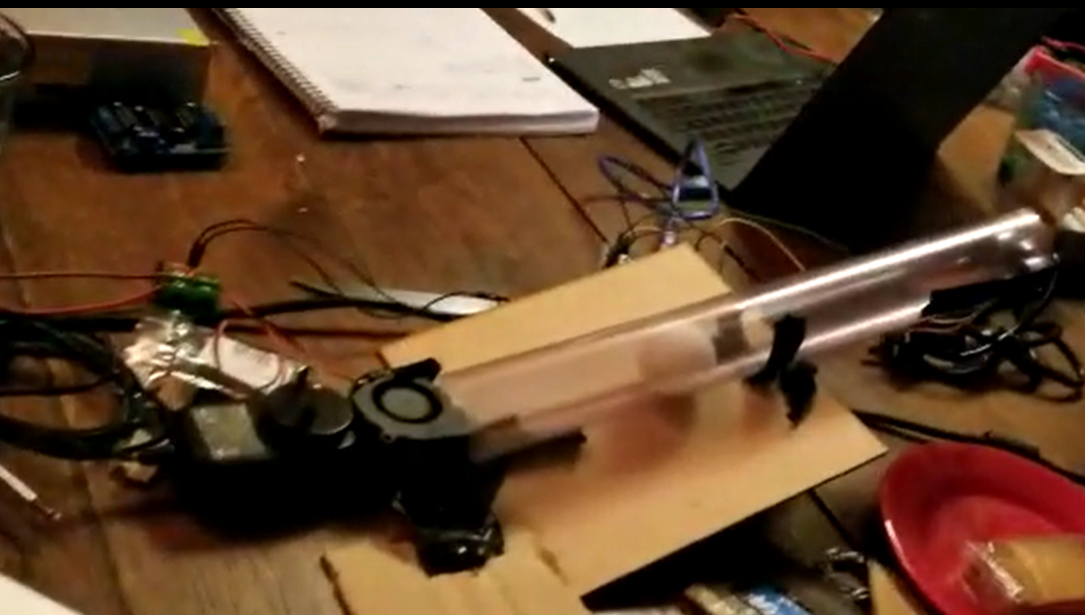
\includegraphics[scale=0.35]{Imagenes/armado.png}
\par\end{centering}

\caption{Imagen del sistema implementado}

\end{figure}
\par\end{center}

\section{Marco Teórico}

Para el modelado físico del sistema se considera que actúan cuatro
fuerzas para la pelota que está dentro del tubo, la fuerza del aire
que empuja a la pelota, la fuerza gravitacional, la fuerza normal del plano y la fricción del plano.
\begin{center}
\begin{figure}[H]
\begin{centering}
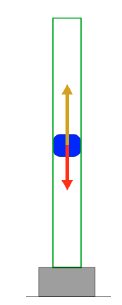
\includegraphics{Imagenes/Fisico.PNG}
\par\end{centering}
\caption{Diagrama de fuerzas de la pelota dentro del tubo}

\end{figure}
\par\end{center}

De la segunda Ley de Newton se tiene que:
\begin{center}
\[
m\frac{d^{2}y}{dt^{2}}=\sum F_{y}
\]
\par\end{center}

\begin{center}
\[
m\frac{d^{2}y}{dt^{2}}=F_{aire}+F_{r}-F_{g_{y}}
\]
\par\end{center}

\begin{center}
\begin{equation}
\frac{d^{2}y}{dt^{2}}=\frac{1}{2m}C_{d}\rho\pi r^{2}(v_{aire}-\frac{dy}{dt})^{2}+\mu g \cdot cos(\theta)-g\cdot sen(\theta)
\end{equation}
\par\end{center}

Donde:
\begin{itemize}
\item $\rho\sim1.2kg/m^{3}$, la densidad volumétrica del aire
\item $m=2.7g$, la masa de la pelota de ping pong
\item $r=2cm$ es el radio de la pelota de ping pong
\item $y$ es la posición vertical de la pelota dentro del tubo
\item $v_{aire}$ es la rapidez promedio del aire cerca de la pelota
\item $g=9.81m/s^{2}$, la constante gravitacional
\item $C_{d}=\frac{24}{Re}+\frac{6}{1+\sqrt{Re}}+0.4$, el coeficiente de
arrastre
\item $Re=\frac{2r\rho(v_{aire}-\frac{dy}{dt})}{\eta}$
\item $\eta$ es la viscosidad dinámica del aire.
\item $\mu$ es el coeficiente de rozamiento del plano.
\end{itemize}
Asumiendo que $Re>1000$ ($C_{d}\thickapprox0.4$) lo cual es válido
si la pelota tiene un radio de 2cm y la velocidad del aire es mayor
a $0.66\frac{m}{seg}$. Entonces la ecuación del problema resulta:
\begin{center}
\begin{equation}
\frac{d^{2}y}{dt^{2}}=\frac{1}{5m}\rho\pi r^{2}(v_{aire}-\frac{dy}{dt})^{2}+\mu g\cdot cos(\theta)-g\cdot sen(\theta) \label{eq:Edo}
\end{equation}
\par\end{center}

Consideramos como la salida del sistema la altura de la pelota de
ping pong con respecto a la base con el ventilador, mientras que la
entrada del sistema es la tensión de continua que fija la velocidad
con la que gira el ventilador de la base. La variable $v_{aire}$
en la ecuación \ref{eq:Edo} está relacionada con la velocidad con
la que gira el ventilador mediante una función matemática desconocida
$v_{aire}=f(y,V_{DC})$.

Debido a la complejidad del modelo, se decidió obtener la transferencia
a lazo abierto del sistema de manera empírica a través de un análisis
de la salida obtenida a partir de una determinada entrada cerca del
punto de equilibrio del sistema. Se puede ver de la ecuación \ref{eq:Edo}
que el sistema no es lineal por lo que se eligió como punto de equilibrio
la altura correspondiente a la mitad del tubo y se trabaja como si
el sistema fuera lineal cerca de dicho punto de equilibrio.

Encontrando la relación lineal entre la tensión proporcionada al ventilador
y su velocidad resultante, es decir, algo de la forma $v_{aire}[m/s]=K_{a}.V_{DC}+cte$,
la ecuación \ref{eq:Edo} quedaría en función de la entrada del sistema
$V_{DC}$.


\subsection{Controlador PID}
\begin{center}
\begin{figure}[H]
\begin{centering}
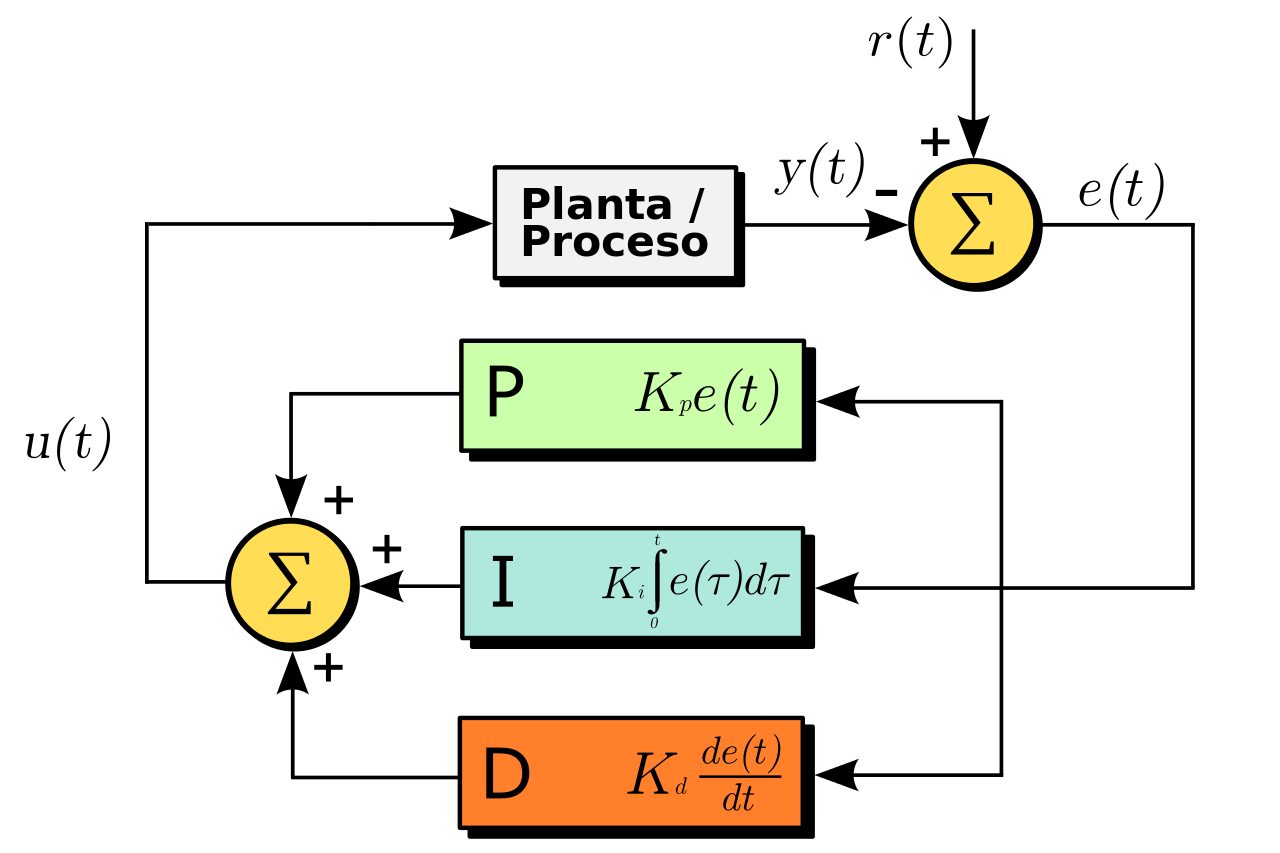
\includegraphics[scale=0.35]{Imagenes/PID_wiki}
\par\end{centering}
\caption{Esquema en bloques del controlador PID.}
\label{fig:pid}
\end{figure}
\par\end{center}

Para controlar la respuesta temporal del sistema se uso un controlador PID como se muestra en el esquema de la figura \ref{fig:pid}. El mismo consiste en la suma de tres términos, el proporcional, el integral y el derivativo. La formula de la salida del sistema controlado esta dada por:
$$u(t)=K_p\cdot e(t) + K_i \int_0 ^t e(\tau) d\tau + K_d \frac{de(t)}{dt}$$
Pero como el control sera aplicado mediante un arduino, la ecuación en realidad se discretiza y queda de la forma:
$$u(nT)=K_p\cdot e(nT) + K_i\cdot \sum_{i=0} ^n \frac{e(iT)+e(iT-T)}{2} T  + K_d \cdot \frac{e(iT)-e(iT-T)}{T}$$

El termino derivativo le agrega ceros al sistema, por lo que cumple la función de cambiar el lugar de raíces. El termino integral agrega un polo en el origen, por lo que aumenta el orden del sistema y sirve para disminuir el error en régimen permanente. Por ultimo, el termino proporcional mueve los polos del sistema dentro del lugar de raíces establecido.
\section{Implementación y resultados}
Dado que la transferencia del modelo linealizado de la planta no es conocida. Se encontraron las constantes del controlador PID efectuando un ajuste manual.
En primer lugar se busco que el sistema oscile utilizando solo un control proporcional, y comenzando con un valor pequeño de $K_p$. Por lo que los valores iniciales utilizados para comenzar el ajuste fueron:
\begin{itemize}
    \item $K_p = 0.1$
    \item $K_i = K_d = 0$
\end{itemize}
Para legar a la oscilación se fue incrementando de manera progresiva el valor de $K_p$ de a saltos de a 0.1, hasta observar una oscilación apreciable. La oscilación se encontró para $K_p = 1.3$, realizando saltos mas pequeños cercanos a ese valor se determino que:
$$K_{oscilación} = K_p = 1.32$$
Una vez conseguido esto, se utilizaron:
\begin{itemize}
    \item $K_p = \frac{K_{oscilación}}{2}=0.66$
    \item $K_i = 0.1$
    \item $K_d = 0$
\end{itemize}
En este nuevo paso, se fue incrementando progresivamente el valor de $K_i$ hasta que visualmente se verifico una respuesta lo mas cercana posible a una respuesta críticamente amortiguada. Esto se consiguió para el valor de:
$$K_d = 0.43$$
Y pro ultimo, para finalizar el ajuste manual se repitió la misma secuencia pero esta vez para $K_d$ y esta vez buscando que el sistema pueda recuperarse de variaciones sin sobrepico apreciable.

Los valores óptimos que se obtuvieron luego del ajuste manual se pueden observar en la tabla \ref{tab:valores_ajuste}.
\begin{table}[h]
    \centering
    \begin{tabular}{|c|c|c|}
        \hline
        $K_p$ & $K_i$ & $K_d$  \\
        \hline
         0.66 & 0.43 & 0.8  \\
         \hline
    \end{tabular}
    \caption{Valores obtenidos luego del ajuste}
    \label{tab:valores_ajuste}
\end{table}
Una vez finalizado el ajuste del controlador, se analizo el funcionamiento del mismo a lo largo de todo el tubo. Con este fin se excito al sistema con un escalón que oscilaba entre 3 niveles, uno cercano a la base del tubo, otro alrededor de la mitad y el ultimo en la parte superior cercana al sensor de distancia. El resultado se puede observar en la figura \ref{fig:resp_temp}, donde el valor mas grande del escalón se corresponde al nivel mas cercano a la base, ya que es el mas lejano al sensor y por eso se encuentra a la mayor distancia del mismo, y el nivel mas bajo al punto mas cercano al sensor.
\begin{center}
\begin{figure}[h]
\begin{centering}
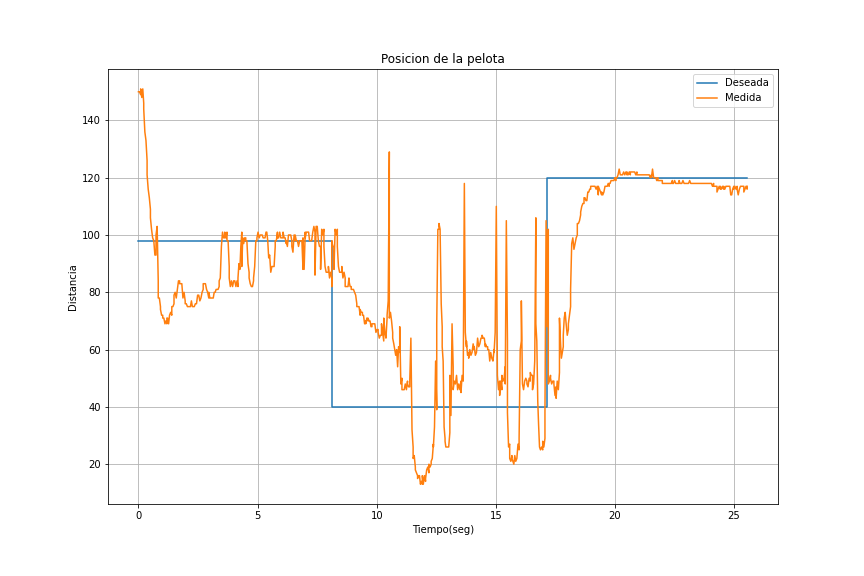
\includegraphics[scale=0.5]{Imagenes/Total.PNG}
\par\end{centering}
\caption{Respuesta temporal del sistema controlado}
\label{fig:resp_temp}
\end{figure}
\par\end{center}

Cada nivel del escalón se mantuvo por 8 segundos antes de realizar la transición al siguiente. Como se puede apreciar en la figura \ref{fig:resp_temp} el peor desempeño se tiene para la distancia de 40, la cual es la mas cercana al sensor de distancia. Mientras que el mejor desempeño se obtiene para la distancia de 120, la cual es la mas lejana al sensor de distancia y mas cercana al ventilador en la base.

Encontramos al menos dos razones por las cuales sucede esto. En primer lugar recordamos que el sistema no es lineal, por lo que el sistema presenta distintas transferencias dependiendo de en que lugar del tubo se realiza la linealizacion y por lo tanto cada una tendrá su propio conjunto óptimo de constantes para el controlador.
Al realizar el ajuste manual de las constantes nos manejamos dentro de una zona entre la base y la mitad del tubo, por lo que es de esperar que los mejores resultados se obtengan para los niveles mas cercanos a la base.
En segundo lugar, los picos que se observan en la figura \ref{fig:resp_arriba} son principalmente debido a ruido del sensor de distancia. El sensor de distancia utilizado emplea un sistema de ecos para medir la distancia.Cuando la pelota esta muy cercana al sensor la precisión de este se degrada y se tiene mucho mas ruido en las mediciones.Por lo que los picos observados no son debido a variaciones fuertes en el movimiento de la pelota sino principalmente al ruido en la medición, que este a su vez dificulta la correcta convergencia. Además de esto, existe una diferencia notable entre la capacidad del ventilador de ejercer fuerza a la pelota al final del tubo con respecto a la base, ya que el ventilador utilizado no es de una gran potencia. Esto a su vez dificulta un poco mas la convergencia mientras mas lejos se este de la base, aunque los picos de ruido parecen ser la principal limitación.
\begin{center}
\begin{figure}[h]
\begin{centering}
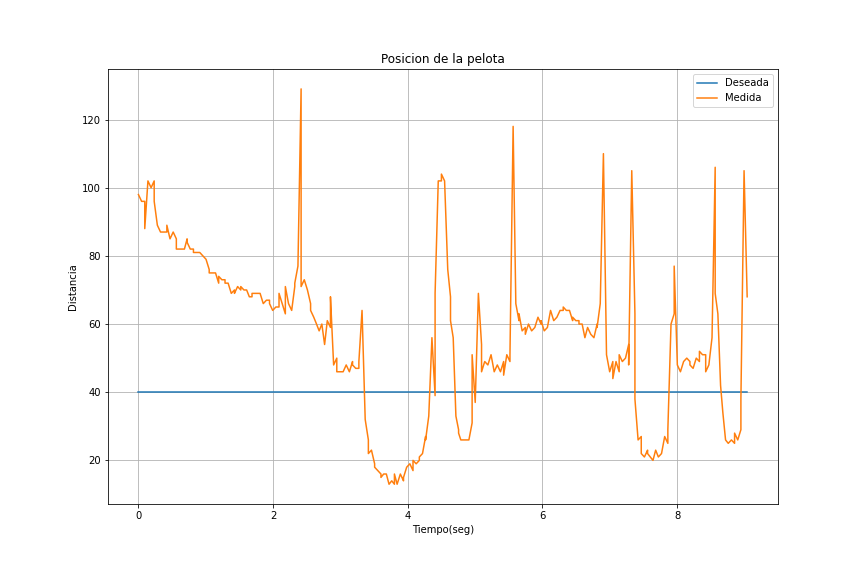
\includegraphics[scale=0.5]{Imagenes/Frame 1.png}
\par\end{centering}
\caption{Respuesta temporal para la zona superior del tubo}
\label{fig:resp_arriba}
\end{figure}
\par\end{center}

Haciendo foco en la sección del tubo con el mejor desempeño, el cual puede verse en la figura \ref{fig:resp_base}. Se tiene que las características de la respuesta temporal controlada son:
\begin{itemize}
    \item $t_{rise}\approx 0.5seg $
    \item $t_{peak} \approx 3.9seg$
\end{itemize}

\begin{center}
\begin{figure}[H]
\begin{centering}
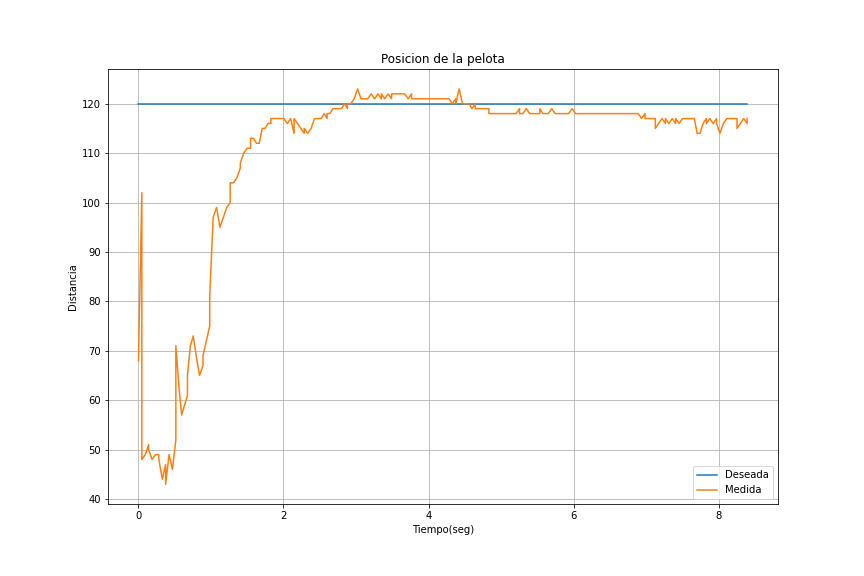
\includegraphics[scale=0.5]{Imagenes/Frame 2.png}
\par\end{centering}
\caption{Respuesta temporal para la zona inferior del tubo}
\label{fig:resp_base}
\end{figure}
\par\end{center}

Por lo que se puede obtener el factor de amortiguamiento del sistema controlado mediante la siguiente ecuación:
$$\xi = cos(\theta)=cos(t_{rise}\cdot w_d)=cos(\frac{t_{rise} \cdot \pi}{t_peak})$$
$$\xi = cos(\frac{0.5 \cdot \pi}{3.9})=0.92$$
El factor de amortiguamiento obtenido es casi 1, lo que se corresponde con la respuesta temporal de la figura \ref{fig:resp_base} ya que el sobrepico es apenas perceptible y se esta muy cerca del caso de una respuesta críticamente amortiguada.




\section{Conclusión}
Para concluir, el problema propuesto de controlar la posicion de una pelota de ping pong sobre un plano inclinado mediante la regulación de velocidad de un ventilador en la base, corresponde a un sistema no lineal. Sin embargo, es posible asumir cierto grado de linealidad dentro de un rango de posiciones en los que se desea trabajar y aplicar algoritmos de control como PID.

En este caso, el ajuste realizado de las constantes del controlador debe realizarse moviéndose dentro de dicho rango, sino se tendrá un mayor error en los resultados obtenidos ya que la transferencia del sistema es considerada valida solo dentro de cierto rango. En esta misma linea, el ventilador y el sensor de distancia tienen un gran impacto en el problema, dado que son los principales componentes que aportan la alinealidad. Se debe garantizar que el ventilador tenga una potencia suficiente para que pueda mover la pelota sin problemas cuando esta se encuentra en la posición mas lejana del rango establecido.
Por ultimo, el sensor de distancia presenta un ruido muy elevado en sus mediciones cuando la pelota se encuentra cerca de el, por lo que es necesario tener esto en cuenta al limitar el rango de posiciones en los que se deseara que se mueva la pelota.
\end{document}
